\chapter{\linIndepTitle}\label{linearind}

Consider a plane $P$ that includes the origin in $\Re^3$ and non-zero vectors $\{u,v,w\}$ in $P$.
\begin{center}
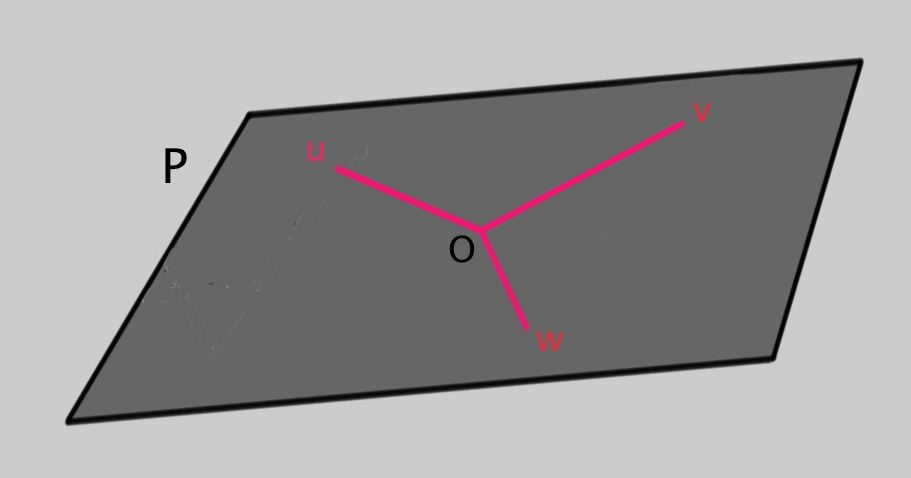
\includegraphics[scale=.3]{\linIndepPath/span_plane.jpg}
\end{center}
If no two of $u, v$ and $w$ are parallel, then $P=\spa \{u,v,w\}$.  But any two vectors determines a plane, so we should be able to span the plane using only two of the vectors $u,v,w$.  Then we could choose two of the vectors in $\{u,v,w\}$ whose span is $P$, and express the other as a linear combination of those two.  Suppose $u$ and $v$ span $P$.  Then there exist constants $d^1, d^2$ (not both zero) such that
$w=d^1u+d^2v$.  Since $w$ can be expressed in terms of $u$ and $v$ we say that it is not independent.
More generally, the relationship
\[
c^1u+c^2v+c^3w=0 \qquad c^i \in \Re, \text{ some $c^i\neq 0$}
\]
expresses the fact that $u,v,w$ are not all independent.

\begin{definition}
\label{independent}
We say that the vectors $v_1, v_2, \ldots, v_n$ are {\bf linearly dependent}\index{Linearly dependent} if there exist constants\footnote{Usually our vector spaces are defined over \(\mathbb{R}\), but in general we can have vector spaces defined over different base fields such as \(\mathbb{C}\) or \(\mathbb{Z}_2\). The coefficients \(c^i\) should come from whatever our base field is (usually \(\mathbb{R}\)).} $c^1, c^2, \ldots, c^n$ not all zero such that
\[
c^1v_1 + c^2v_2+ \cdots +c^nv_n=0.
\]
Otherwise, the vectors $v_1, v_2, \ldots, v_n$ are {\bf linearly independent.}\index{Linearly independent} 
\end{definition}

\begin{remark}
The zero vector $0_V$ can {\it never} be on a list of independent vectors because $\alpha 0_V=0_V$ for any scalar $\alpha$.
\end{remark}

\begin{example}
Consider the following vectors in \(\Re^3\):
\[
v_1=\colvec{4\\-1\\3}, \qquad
v_2=\colvec{-3\\7\\4}, \qquad
v_3=\colvec{5\\12\\17}, \qquad
v_4=\colvec{-1\\1\\0}.
\]
Are these vectors linearly independent?

No, since \(3v_1+2v_2-v_3+v_4=0\), the vectors are linearly {\it dependent}.
\end{example}

\Videoscriptlink{linear_independence_example.mp4}{Worked Example}{linear_independence_example}

\section{Showing Linear Dependence}
In the above example we were given the linear combination \(3v_1+2v_2-v_3+v_4\) seemingly by magic. The next example shows how to find such a linear combination, if it exists.

\begin{example}
Consider the following vectors in $\Re^3$:
\[
v_1=\colvec{0\\0\\1}, 
\qquad v_2=\colvec{1\\2\\1},
\qquad v_3=\colvec{1\\2\\3}.
\]
Are they linearly independent?

We need to see whether the system 
\[
c^1v_1 + c^2v_2+ c^3v_3=0
\]
has any solutions for $c^1, c^2, c^3$.  We can rewrite this as a homogeneous system by building a matrix whose columns are the vectors $v_1$, $v_2$ and $v_3$:
\[
\rowvec{v_1&v_2&v_3}\colvec{c^1\\c^2\\c^3}=0.
\]
This system has solutions if and only if the matrix $M=\rowvec{v_1&v_2&v_3}$ is singular, so we should find the determinant of $M$:
\[
\det M = \det \begin{pmatrix}
0 & 1 & 1 \\
0 & 2 & 2 \\
1 & 1 & 3 \\
\end{pmatrix}
= \det \begin{pmatrix}
1 & 1 \\
2 & 2 \\
\end{pmatrix}
=0.
\]

Therefore nontrivial solutions exist.  At this point we know that the vectors are linearly dependent.  If we need to, we can find coefficients that demonstrate linear dependence by solving
\[
\begin{amatrix}{3}
0 & 1 & 1 & 0\\
0 & 2 & 2 & 0\\
1 & 1 & 3 & 0\\
\end{amatrix} \sim
\begin{amatrix}{3}
1 & 1 & 3 & 0\\
0 & 1 & 1 & 0\\
0 & 0 & 0 & 0\\
\end{amatrix} \sim
\begin{amatrix}{3}
1 & 0 & 2 & 0\\
0 & 1 & 1 & 0\\
0 & 0 & 0 & 0\\
\end{amatrix}.
\]
The solution set  $\{ \mu ( -2,-1,1) ~| ~\mu \in \mathbb{R} \}$ encodes the linear combinations equal to zero;  any choice of $\mu$ will produce coefficients $c^1,c^2,c^3$ that satisfy the linear homogeneous equation.  
In particular, $\mu=1$ corresponds to the equation
\[
c^1v_1 + c^2v_2+ c^3v_3=0 
\Rightarrow -2v_1 - v_2 + v_3=0.
\]
\end{example}

\Reading{LinearIndependence}{1}
%\begin{center}\href{\webworkurl ReadingHomework16/1/}{Reading homework: problem \ref{linearind}.1}\end{center}

\begin{definition}
Any sum of vectors $v_1,\ldots, v_k$ multiplied by scalars $c^1,\ldots,c^k$, namely
$$
c^1 v_1+\cdots + c^k v_k\, ,
$$
is called a {\it linear combination}\index{Linear combination} of $v_1,\ldots , v_k$.
\end{definition}

\begin{theorem}[Linear Dependence]\index{Linear dependence theorem}
\label{linear_dependence}
An ordered set of non-zero vectors $( v_1, \ldots, v_n )$ is linearly dependent if and only if one of the vectors $v_k$ is expressible as a linear combination of the preceding vectors.
\end{theorem}

\begin{proof}
The theorem is an if and only if statement, so there are two things to show.

\begin{itemize}
\item[$i.$]  First, we show that if $v_k=c^1v_1+\cdots c^{k-1}v_{k-1}$ then the set is linearly dependent.

This is easy.  We just rewrite the assumption:
\[
c^1v_1+\cdots+c^{k-1}v_{k-1}-v_k + 0v_{k+1}+\cdots +0v_n=0.
\]
This is a vanishing linear combination of the vectors $\{ v_1, \ldots, v_n \}$ with not all coefficients equal to zero, so $\{ v_1, \ldots, v_n \}$ is a linearly dependent set.
 
\item[$ii.$]  Now we show that linear dependence implies that there exists $k$ for which $v_k$ is a linear combination of the vectors $\{ v_1, \ldots, v_{k-1} \}$.

The assumption says that
\[
c^1v_1 + c^2v_2+ \cdots +c^nv_n=0.
\]
Take $k$ to be the largest number for which $c_k$ is not equal to zero.  So:
\[
c^1v_1 + c^2v_2+ \cdots +c^{k-1}v_{k-1}+c^kv_k=0.
\]

(Note that $k>1$, since otherwise we would have $c^1v_1=0\Rightarrow v_1=0$, contradicting the assumption that none of the $v_i$ are the zero vector.)

So we can rearrange the equation:
\begin{eqnarray*}
c^1v_1 + c^2v_2+ \cdots +c^{k-1}v_{k-1}&=&-c^kv_k\\ \Rightarrow\ 
-\frac{c^1}{c^k}v_1 - \frac{c^2}{c^k}v_2 - \cdots -\frac{c^{k-1}}{c^k}v_{k-1}&=&v_k.
\end{eqnarray*}

Therefore we have expressed $v_k$ as a linear combination of the previous vectors, and we are done.
\end{itemize}
\end{proof}

\Videoscriptlink{linear_independence_thm.mp4}{Worked proof}{scripts_linear_independence_thm}

\begin{example}
Consider the vector space $P_2(t)$ of polynomials of degree less than or equal to $2$.  Set:
\begin{eqnarray*}
v_1 &=& 1+t \\
v_2 &=& 1+t^2 \\
v_3 &=& t+t^2 \\
v_4 &=& 2+t+t^2 \\
v_5 &=& 1+t+t^2. \\
\end{eqnarray*}
The set $\{ v_1, \ldots, v_5 \}$ is linearly dependent, because $v_4 = v_1+v_2$.  
\end{example}

\section{Showing Linear Independence} 
We have seen two different ways to show a set of vectors is linearly dependent: we can either find a linear combination of the vectors which is equal to zero, or we can express one of the vectors as a linear combination of the other vectors. On the other hand, to check that a set of vectors is linearly {\it independent}, we must check that every  linear combination of our vectors with non-vanishing coefficients gives something other than the zero vector. Equivalently, to show that the set \(v_1, v_2, \ldots, v_n\) is linearly independent, we must show that the equation \(c_1 v_1+c_2v_2 + \cdots + c_n v_n=0\) has no solutions other than \(c_1=c_2=\cdots=c_n=0.\)

\begin{example}
Consider the following vectors in $\Re^3$:
\[
v_1=\colvec{0\\0\\2},
\qquad v_2=\colvec{2\\2\\1},
\qquad v_3=\colvec{1\\4\\3}.
\]
Are they linearly independent?

We need to see whether the system
\[
c^1v_1 + c^2v_2+ c^3v_3=0
\]
has any solutions for $c^1, c^2, c^3$.  We can rewrite this as a homogeneous system:
\[
\rowvec{v_1&v_2&v_3}\colvec{c^1\\c^2\\c^3}=0.
\]
This system has solutions if and only if the matrix $M=\rowvec{v_1&v_2&v_3}$ is singular, so we should find the determinant of $M$:
\[
\det M = \det \begin{pmatrix}
0 & 2 & 1 \\
0 & 2 & 4 \\
2 & 1 & 3 \\
\end{pmatrix}
= 2 \det \begin{pmatrix}
2 & 1 \\
2 & 4 \\
\end{pmatrix}
=12.
\]
Since the matrix \(M\) has non-zero determinant, the only solution to the system of equations
\[
\rowvec{v_1&v_2&v_3}\colvec{c^1\\c^2\\c^3}=0
\]
is \(c_1=c_2=c_3=0\). So the vectors \(v_1, v_2, v_3\) are linearly independent.
\end{example}

Here is another example with bits:

\begin{example}
Let $\mathbb{Z}_2^3$ be the space of $3\times 1$ bit-valued matrices (i.e., column vectors).  Is the following subset linearly independent?
\[
\left\{ \colvec{1\\1\\0}, \colvec{1\\0\\1}, 
\colvec{0\\1\\1} \right\}
\]

If the set is linearly dependent, then we can find non-zero solutions to the system:
\[
c^1\colvec{1\\1\\0}+ c^2 \colvec{1\\0\\1} 
+c^3 \colvec{0\\1\\1}=0,
\]
which becomes the linear system
\[
\begin{pmatrix}
1 & 1 & 0 \\
1 & 0 & 1 \\
0 & 1 & 1 \\
\end{pmatrix}\colvec{c^1\\c^2\\c^3}=0.
\]
Solutions exist if and only if the determinant of the matrix is non-zero.  But:
\[
\det \begin{pmatrix}
1 & 1 & 0 \\
1 & 0 & 1 \\
0 & 1 & 1 \\
\end{pmatrix} = 1 \det \begin{pmatrix}
0 & 1 \\
1 & 1 \\
\end{pmatrix} -1 \det \begin{pmatrix}
1 & 1 \\
0 & 1 \\
\end{pmatrix} = -1-1=1+1=0
\]
Therefore non-trivial solutions exist, and the set is not linearly independent.

\end{example}


\Reading{LinearIndependence}{2}
%\begin{center}\href{\webworkurl ReadingHomework16/2/}{Reading homework: problem \ref{linearind}.2}\end{center}

\section{From Dependent Independent } 
Now suppose vectors 
$v_1,\ldots, v_n$ are linearly dependent, 
\[
c^1v_1 + c^2v_2+ \cdots +c^nv_n=0
\]
with $c^1\neq 0$.  Then:
\[
\spa \{v_1,\ldots, v_n\} = \spa \{ v_2,\ldots, v_n\}
\]
because any $x\in \spa \{v_1,\ldots, v_n\}$ is given by
\begin{eqnarray*}
x &=& a^1v_1 + \cdots+ a^nv_n \\
&=& a^1\left( -\frac{c^2}{c_1}v_2- \cdots -\frac{c^n}{c_1}v_n \right) + a^2v_2 + \cdots + a^nv_n \\
&=& \left(a^2-a^1\frac{c^2}{c_1}\right)v_2 + \cdots + \left(a^n-a^1\frac{c^n}{c_1}\right)v_n.
\end{eqnarray*}
Then $x$ is in $\spa \{v_2,\ldots, v_n\}$.

When we write a vector space as the span of a list of vectors, we would like that list to be as short as possible (this idea is explored further in \hyperref[dimension]{chapter~\ref*{sec:dimension}}).
This can be achieved by iterating the above procedure.

\begin{example}
In the above example, we found that $v_4=v_1+v_2$.  In this case, any expression for a vector as a linear combination involving $v_4$ can be turned into a combination without $v_4$ by making the substitution $v_4=v_1+v_2$.

Then:
\begin{eqnarray*}
S &=& \spa \{ 1+t , 1+t^2, t+t^2, 2+t+t^2, 1+t+t^2 \} \\
&=& \spa \{ 1+t , 1+t^2, t+t^2, 1+t+t^2 \}.
\end{eqnarray*}
Now we notice that $1+t+t^2=\frac{1}{2}(1+t) +\frac{1}{2}(1+t^2) + \frac{1}{2}(t+t^2)$.  So the vector $1+t+t^2=v_5$ is also extraneous, since it can be expressed as a linear combination of the remaining three vectors, $v_1, v_2,v_3$.  Therefore 
\[
S = \spa \{ 1+t , 1+t^2, t+t^2 \}.
\]

In fact, you can check that there are no (non-zero) solutions to the linear system
\[
c^1(1+t) + c^2(1+t^2) + c^3(t+t^2)=0.
\]
Therefore the remaining vectors $\{ 1+t , 1+t^2, t+t^2 \}$ are linearly independent, and span the vector space $S$.  Then these vectors are a minimal spanning set\index{Minimal spanning set}, in the sense that no more vectors can be removed since the vectors are linearly independent.
Such a set is called a \emph{basis}\index{Basis!example of} for $S$.
\end{example}





%To summarize, the key definition in this lecture was:
%\begin{center}
%
\includegraphics[scale=.3]{\linIndepPath/linear_dependent.jpg}
%\end{center}
%Perhaps the most useful Theorem was:
%\begin{center}
%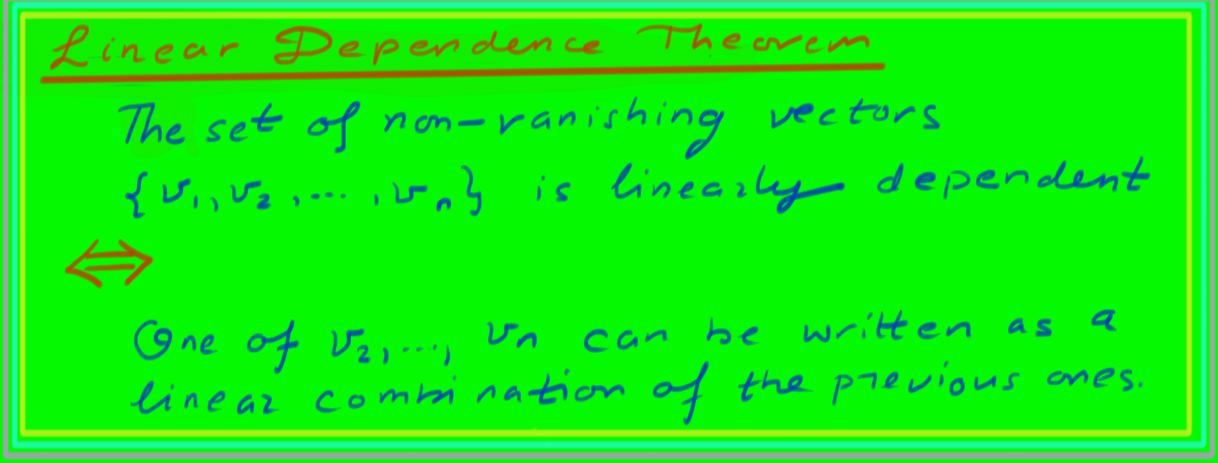
\includegraphics[scale=.3]{\linIndepPath/linear_dependence_thm.jpg}
%\end{center}

%\section*{References}
%Hefferon, Chapter Two, Section II: Linear Independence
%\\
%Hefferon, Chapter Two, Section III.1: Basis
%\\
%Beezer, Chapter V, Section LI
%\\
%Beezer, Chapter V, Section LDS
%\\
%Beezer, Chapter VS, Section LISS, Subsection LI
%\\
%Wikipedia:
%\begin{itemize}
%\item \href{http://en.wikipedia.org/wiki/Linear_independence}{Linear Independence}
%\item \href{http://en.wikipedia.org/wiki/Basis_(linear_algebra)}{Basis}
%\end{itemize}

\section{Review Problems}
{\bf Webwork:} 
\begin{tabular}{|c|c|}
\hline
Reading Problems & 
 \hwrref{LinearIndependence}{1},\hwrref{LinearIndependence}{2}\\
 Testing for linear independence &\hwref{LinearIndependence}{3},
 \hwref{LinearIndependence}{4}\\
 Gaussian elimination &\hwref{LinearIndependence}{5}\\
 Spanning and linear independence &\hwref{LinearIndependence}{6}\\
  \hline
\end{tabular}




\begin{enumerate}

\item While performing  Gaussian elimination on these augmented matrices write the full system of equations describing the new rows in terms of the old rows above each equivalence symbol as in  \hyperlink{Keeping track of EROs with equations between rows}{Example}~\ref{Rsystem}. 
$$
\begin{amatrix}{2} 
2 & 2 & 10 \\
1 & 2 & 8 \\
\end{amatrix}
,~
\begin{amatrix}{3} 
1 & 1 & 0 & 5 \\
1 & 1 & \!\!-1& 11 \\
-1 & 1 & 1 & -5 \\ 
\end{amatrix}
$$

%%%%%%%%%%%%%%%%%%%

\item Solve the vector equation by applying ERO matrices to each side of the equation to perform elimination. Show each matrix explicitly as in \hyperlink{Undoing}{Example~\ref{slowly}}.

\begin{eqnarray*}
\begin{pmatrix}
3	&6 	&2 \\ %-3
5 	&9 	&4 \\ %1
2	&4	&2 \\ %0
\end{pmatrix} 
\begin{pmatrix}
 x \\ 
y \\
z 
\end{pmatrix} 
=
\begin{pmatrix}
-3 \\ 
1  \\
0  \\
\end{pmatrix} 
\end{eqnarray*}

%%%%%%%%%%%%%%%%%%%

\item Solve this vector equation by finding the inverse of the matrix through $(M|I)\sim (I|M^{-1})$ and then applying $M^{-1}$ to both sides of the equation. 
\begin{eqnarray*}
\begin{pmatrix}
2	&1 	&1 \\ %9
1 	&1 	&1 \\ %6
1	&1	&2 \\ %7
\end{pmatrix} 
\begin{pmatrix}
 x \\ 
y \\
z 
\end{pmatrix} 
=
\begin{pmatrix}
9 \\ 
6  \\
7  \\
\end{pmatrix} 
\end{eqnarray*}


%%%%%%%%%%%%%%%%%%%

\item Follow the method of  \hyperlink{elldeeeww}{Examples~\ref{factorize} and~\ref{factorizes}} to find the $LU$ and $LDU$ factorization of 
\begin{eqnarray*}
\begin{pmatrix}
3	&3 	&6 \\ %0 %2
3 	&5 	&2 \\ %1 %1
6	&2	&5 \\ %0 %1
\end{pmatrix} .
\end{eqnarray*}



%%%%%%%%%%%%%%%%%%%%

\item 
Multiple matrix equations with the same matrix can be solved simultaneously. 
\begin{enumerate}
\item Solve both systems by performing elimination on just one augmented matrix.
\begin{eqnarray*}
\begin{pmatrix}
2	&-1 	&-1 \\ %0 %2
-1 	&1 	&1 \\ %1 %1
1	&-1	&0 \\ %0 %1
\end{pmatrix} 
\begin{pmatrix}
 x \\ 
y \\
z 
\end{pmatrix} 
=
\begin{pmatrix}
0\\ 
1  \\
0  \\
\end{pmatrix} 
,~
\begin{pmatrix}
2	&-1 	&-1 \\ %0 %2
-1 	&1 	&1 \\ %1 %1
1	&-1	&0 \\ %0 %1
\end{pmatrix} 
\begin{pmatrix}
 a \\ 
b \\
c 
\end{pmatrix} 
=
\begin{pmatrix}
2\\ 
1  \\
1  \\
\end{pmatrix} 
\end{eqnarray*}
\item Give an interpretation of the columns of $M^{-1}$ in $(M|I)\sim (I|M^{-1})$ in terms of solutions to certain systems of linear equations.
\end{enumerate}

%%%%%%%%%%%%%%%%%%%%%%%%

\item How can you convince your fellow students to never make this mistake?
\begin{eqnarray*}
\begin{amatrix}{3} 
1 & 0 & 2 & 3 \\ 
0 & 1 & 2& 3 \\
2 & 0 & 1 & 4 \\
\end{amatrix} 
& 
\stackrel{R_1'=R_1+R_2}{
\stackrel{R_2'=R_1-R_2}{ 
\stackrel{\ R_3'= R_1+2R_2}{\sim}}}
&
\begin{amatrix}{3} 
1 & 1 & 4 & 6 \\
1 & \!\!-1 & 0& 0 \\
1 & 2 & 6 & 9 
\end{amatrix}
\end{eqnarray*}

\item Is $LU$ factorization of a matrix unique?  Justify your answer.


\item[$\infty$.] If you randomly create a matrix by picking numbers out of the blue, it will probably be difficult to perform elimination or factorization; fractions and large numbers will probably be involved. To invent simple problems it is better to start with a simple answer:
\begin{enumerate}
\item Start with any augmented matrix in RREF. Perform EROs to make most of the components non-zero. Write the result on a separate piece of paper and give it to your friend. Ask that friend to find RREF of the augmented matrix you gave them. Make sure they get the same augmented matrix you started with.  
\item Create  an upper triangular matrix $U$ and a lower triangular matrix~$L$ with only $1$s on the diagonal. Give the result to a friend to factor into $LU$ form. 
\item Do the same with an $LDU$ factorization. 
\end{enumerate}
\end{enumerate}

\phantomnewpage




